\documentclass[]{article}
\usepackage[T1]{fontenc}
\usepackage{lmodern}
\usepackage{amssymb,amsmath}
\usepackage{ifxetex,ifluatex}
\usepackage{fixltx2e} % provides \textsubscript
% Set line spacing
% use upquote if available, for straight quotes in verbatim environments
\IfFileExists{upquote.sty}{\usepackage{upquote}}{}
\ifnum 0\ifxetex 1\fi\ifluatex 1\fi=0 % if pdftex
  \usepackage[utf8]{inputenc}
\else % if luatex or xelatex
  \ifxetex
    \usepackage{mathspec}
    \usepackage{xltxtra,xunicode}
  \else
    \usepackage{fontspec}
  \fi
  \defaultfontfeatures{Mapping=tex-text,Scale=MatchLowercase}
  \newcommand{\euro}{€}
\fi
% use microtype if available
\IfFileExists{microtype.sty}{\usepackage{microtype}}{}
\usepackage[margin=1in]{geometry}
\usepackage{color}
\usepackage{fancyvrb}
\newcommand{\VerbBar}{|}
\newcommand{\VERB}{\Verb[commandchars=\\\{\}]}
\DefineVerbatimEnvironment{Highlighting}{Verbatim}{commandchars=\\\{\}}
% Add ',fontsize=\small' for more characters per line
\usepackage{framed}
\definecolor{shadecolor}{RGB}{248,248,248}
\newenvironment{Shaded}{\begin{snugshade}}{\end{snugshade}}
\newcommand{\KeywordTok}[1]{\textcolor[rgb]{0.13,0.29,0.53}{\textbf{{#1}}}}
\newcommand{\DataTypeTok}[1]{\textcolor[rgb]{0.13,0.29,0.53}{{#1}}}
\newcommand{\DecValTok}[1]{\textcolor[rgb]{0.00,0.00,0.81}{{#1}}}
\newcommand{\BaseNTok}[1]{\textcolor[rgb]{0.00,0.00,0.81}{{#1}}}
\newcommand{\FloatTok}[1]{\textcolor[rgb]{0.00,0.00,0.81}{{#1}}}
\newcommand{\CharTok}[1]{\textcolor[rgb]{0.31,0.60,0.02}{{#1}}}
\newcommand{\StringTok}[1]{\textcolor[rgb]{0.31,0.60,0.02}{{#1}}}
\newcommand{\CommentTok}[1]{\textcolor[rgb]{0.56,0.35,0.01}{\textit{{#1}}}}
\newcommand{\OtherTok}[1]{\textcolor[rgb]{0.56,0.35,0.01}{{#1}}}
\newcommand{\AlertTok}[1]{\textcolor[rgb]{0.94,0.16,0.16}{{#1}}}
\newcommand{\FunctionTok}[1]{\textcolor[rgb]{0.00,0.00,0.00}{{#1}}}
\newcommand{\RegionMarkerTok}[1]{{#1}}
\newcommand{\ErrorTok}[1]{\textbf{{#1}}}
\newcommand{\NormalTok}[1]{{#1}}
\usepackage{graphicx}
% Redefine \includegraphics so that, unless explicit options are
% given, the image width will not exceed the width of the page.
% Images get their normal width if they fit onto the page, but
% are scaled down if they would overflow the margins.
\makeatletter
\def\ScaleIfNeeded{%
  \ifdim\Gin@nat@width>\linewidth
    \linewidth
  \else
    \Gin@nat@width
  \fi
}
\makeatother
\let\Oldincludegraphics\includegraphics
{%
 \catcode`\@=11\relax%
 \gdef\includegraphics{\@ifnextchar[{\Oldincludegraphics}{\Oldincludegraphics[width=\ScaleIfNeeded]}}%
}%
\ifxetex
  \usepackage[setpagesize=false, % page size defined by xetex
              unicode=false, % unicode breaks when used with xetex
              xetex]{hyperref}
\else
  \usepackage[unicode=true]{hyperref}
\fi
\hypersetup{breaklinks=true,
            bookmarks=true,
            pdfauthor={Henry Scharf},
            pdftitle={moving from for to foreach},
            colorlinks=true,
            citecolor=blue,
            urlcolor=blue,
            linkcolor=magenta,
            pdfborder={0 0 0}}
\urlstyle{same}  % don't use monospace font for urls
\setlength{\parindent}{0pt}
\setlength{\parskip}{6pt plus 2pt minus 1pt}
\setlength{\emergencystretch}{3em}  % prevent overfull lines
\setcounter{secnumdepth}{0}

%%% Change title format to be more compact
\usepackage{titling}
\setlength{\droptitle}{-2em}
  \title{moving from for to foreach}
  \pretitle{\vspace{\droptitle}\centering\huge}
  \posttitle{\par}
  \author{Henry Scharf}
  \preauthor{\centering\large\emph}
  \postauthor{\par}
  \predate{\centering\large\emph}
  \postdate{\par}
  \date{December 4, 2014}




\begin{document}

\maketitle


{
\hypersetup{linkcolor=black}
\setcounter{tocdepth}{2}
\tableofcontents
}
\section{why?}\label{why}

\subsection{embarassingly parallel
tasks}\label{embarassingly-parallel-tasks}

These are computational tasks which involve many separate, independently
executable calculations. Some common statistical examples of
embarassingly {\textbf{parallel}} processes:

\begin{itemize}
\itemsep1pt\parskip0pt\parsep0pt
\item
  bootstrapping
\item
  cross-validation
\item
  simulating independent random variables (\texttt{dorng})
\end{itemize}

In contrast, some sequential or {\textbf{non-parallel}} processes:

\begin{itemize}
\itemsep1pt\parskip0pt\parsep0pt
\item
  MCMC algorithms
\item
  several types of model selection (e.g.: \texttt{step()} or the LARS
  algorithm for LASSO)
\end{itemize}

\texttt{for} loops that do not explicitly involve dependent calculations
are wasteful if we have multiple processors available. Perhaps even
worse, the time cost of using such an approach can put some useful
statistical tools beyond our reach!

\subsection{options}\label{options}

\begin{itemize}
\itemsep1pt\parskip0pt\parsep0pt
\item
  Changing from a for loop to one of the \texttt{apply()} functions can
  help, but still doesn't use multiple processors.
\item
  Use the \texttt{parallel} package (thanks, Miranda!).
\item
  Don't use R.
\item
  Use the \texttt{foreach} package!
\end{itemize}

\subsection{why foreach?}\label{why-foreach}

We would like to find a way to make use of our whole computer, and make
valuable tasks like bootstrapping available, but without having to
invest large amounts of time in learning new programming languages.
Enter \texttt{foreach}, which keeps the structure of a for loop, but
allows us to drop two key assumptions:

\begin{itemize}
\itemsep1pt\parskip0pt\parsep0pt
\item
  sequentiality
\item
  single processor architecture
\end{itemize}

{\textbf{Our goal}}: We will begin with a simple chunk of R code
involving a for loop and transform it into a \texttt{foreach} loop.
Along the way, we'll take a look at the equivalent computation done with
an \texttt{apply()} function, and see that using \texttt{foreach} and
multiple processors outperforms this.

\section{example: data and research
question}\label{example-data-and-research-question}

We are going to look at data from the New York City bikeshare program
\href{https://www.citibikenyc.com/}{Citibike}.

\begin{itemize}
\itemsep1pt\parskip0pt\parsep0pt
\item
  7 busiest locations from May 2014
\item
  response: \# of arrivals each hour of every day in the month
\item
  covariates: hour of the day and whether the day is a weekend
\end{itemize}

One of the costliest parts of operating a bike share program comes from
the finiteness of the bicycle stations. A station can only hold so many
bicycles, and a full (empty) station means customers cannot drop off
(pick up) a bike. Thus, managers are forced to use trucks to manually
redistribute bicycles.

We want to find a model which can offer good prediction, with the hope
that this will inform our plans for future station locations/sizes. For
this example, we start with a few plausible models and use K-fold cross
validation to decide which one to use.

\subsection{locations of our 7 sites}\label{locations-of-our-7-sites}

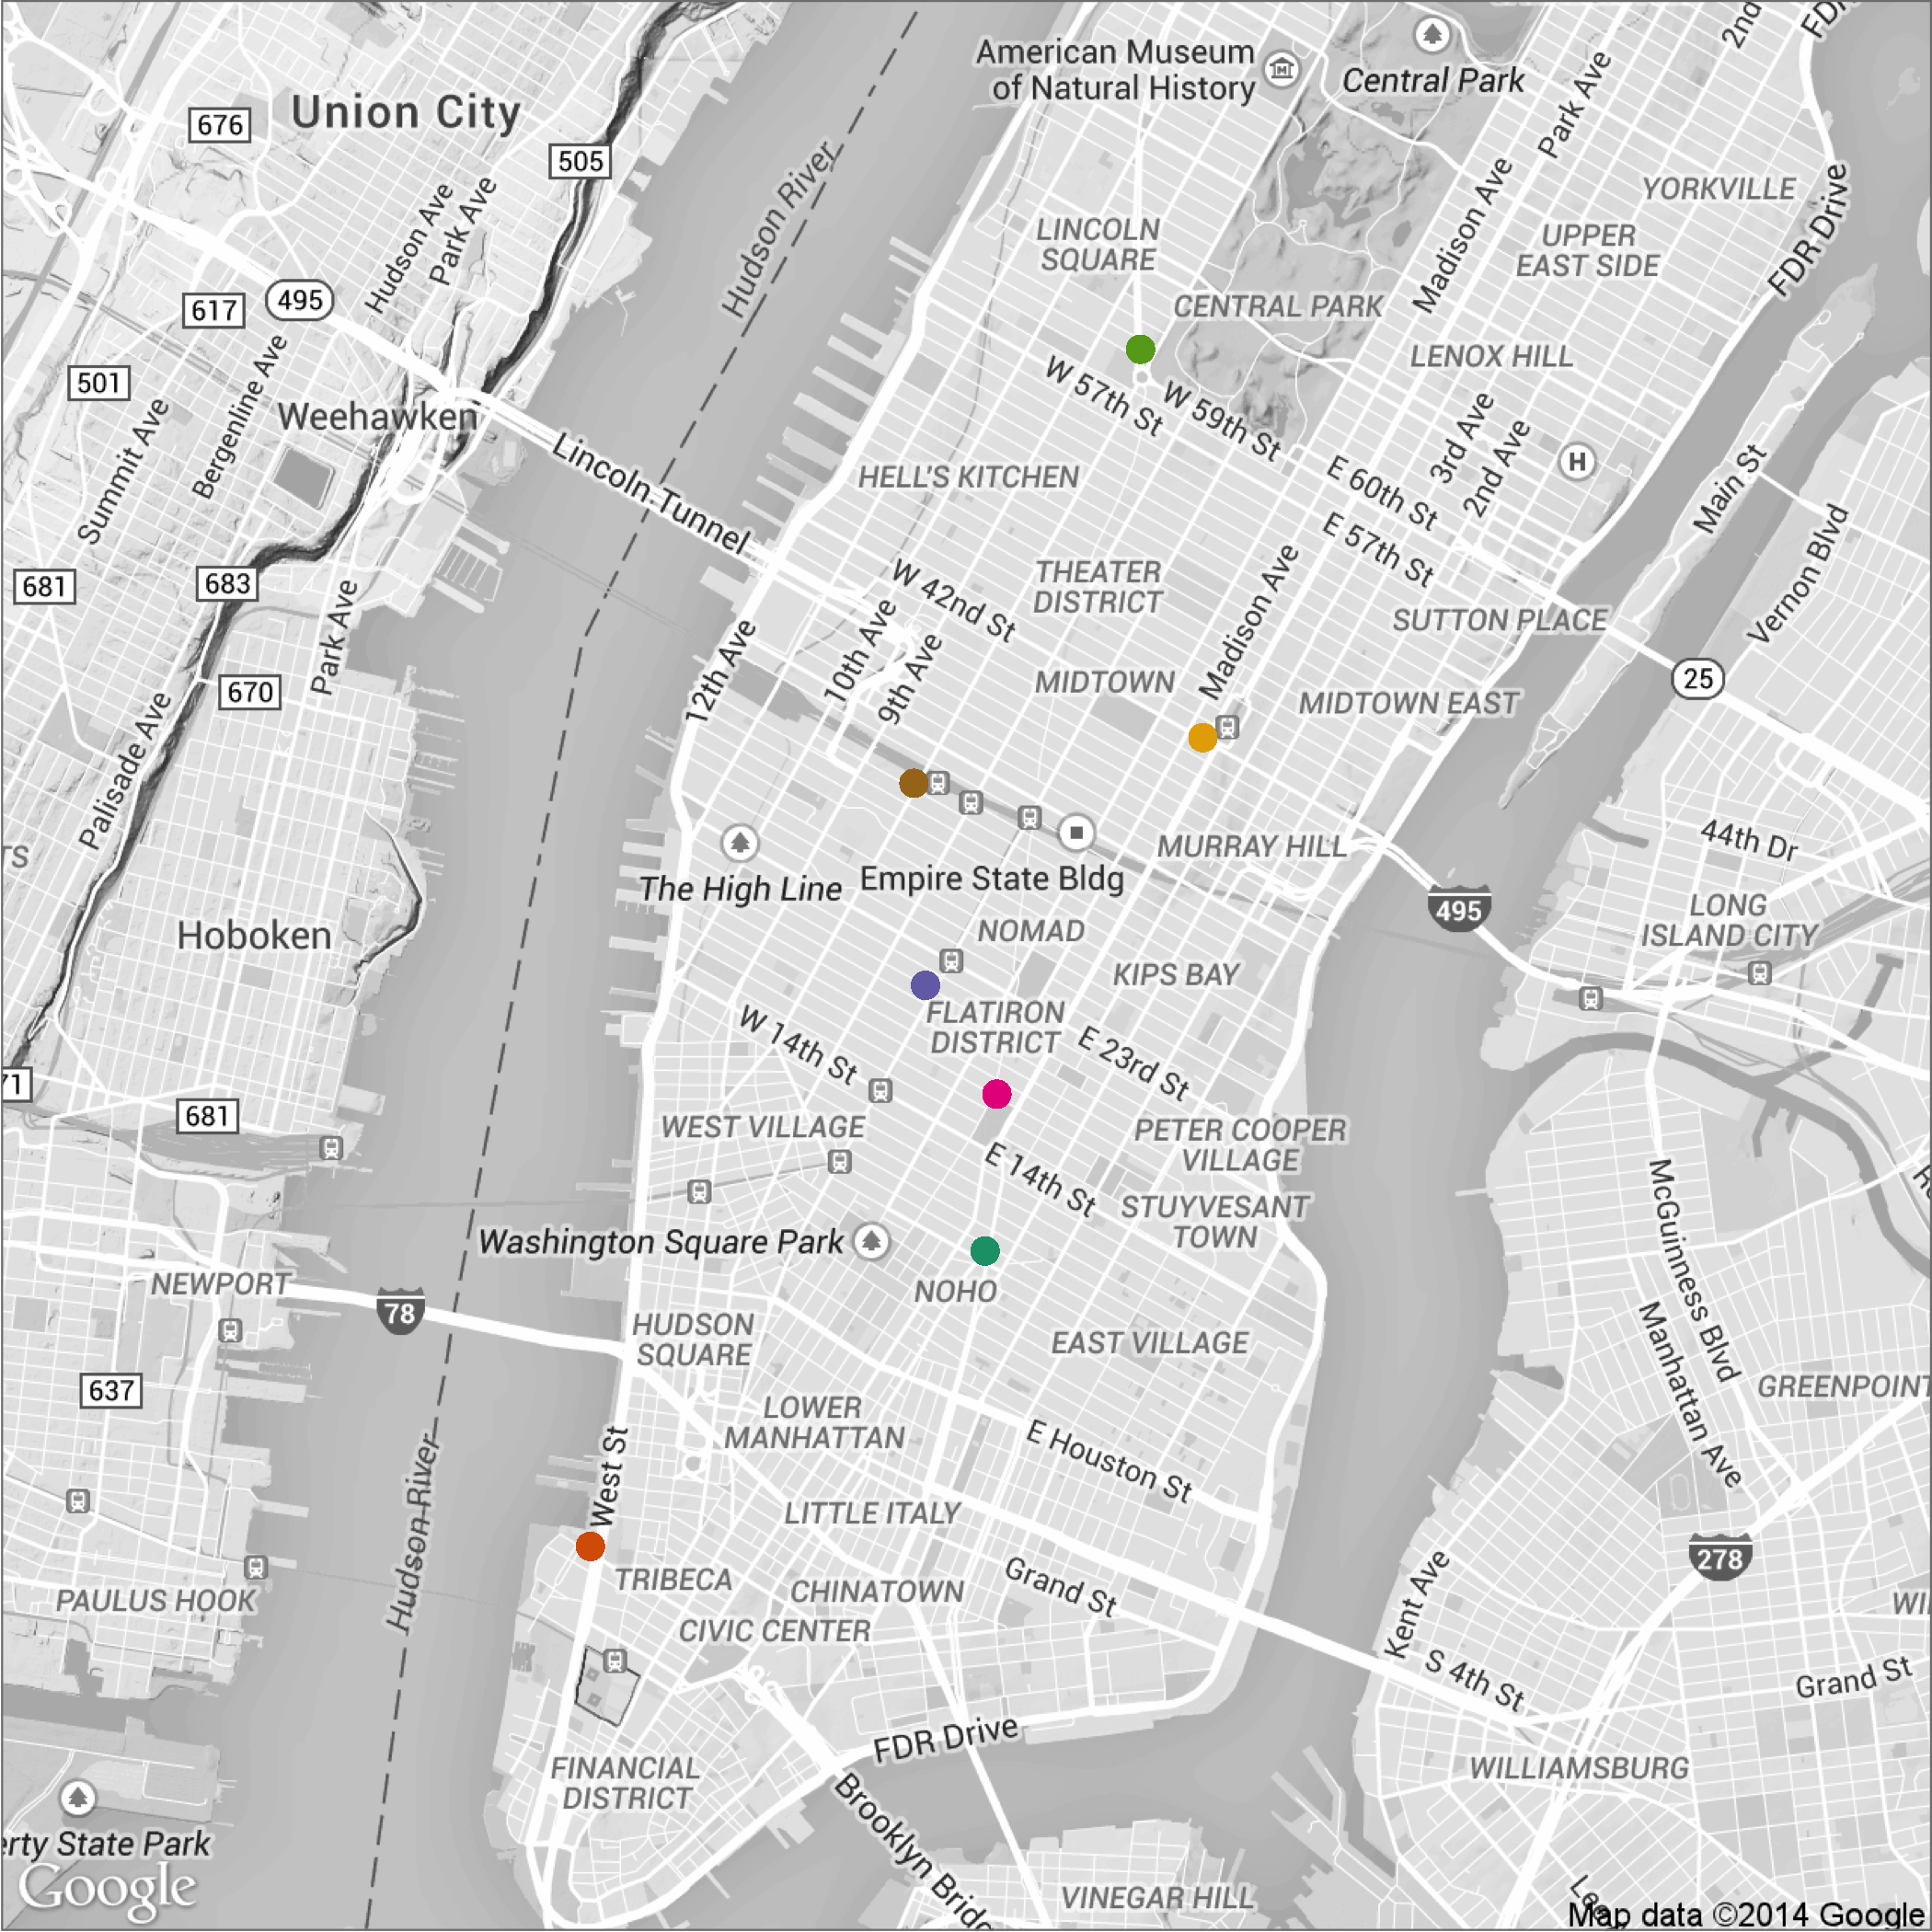
\includegraphics{../fig/map_top7.png}

\begin{center}\rule{0.5\linewidth}{\linethickness}\end{center}

\subsection{data}\label{data}

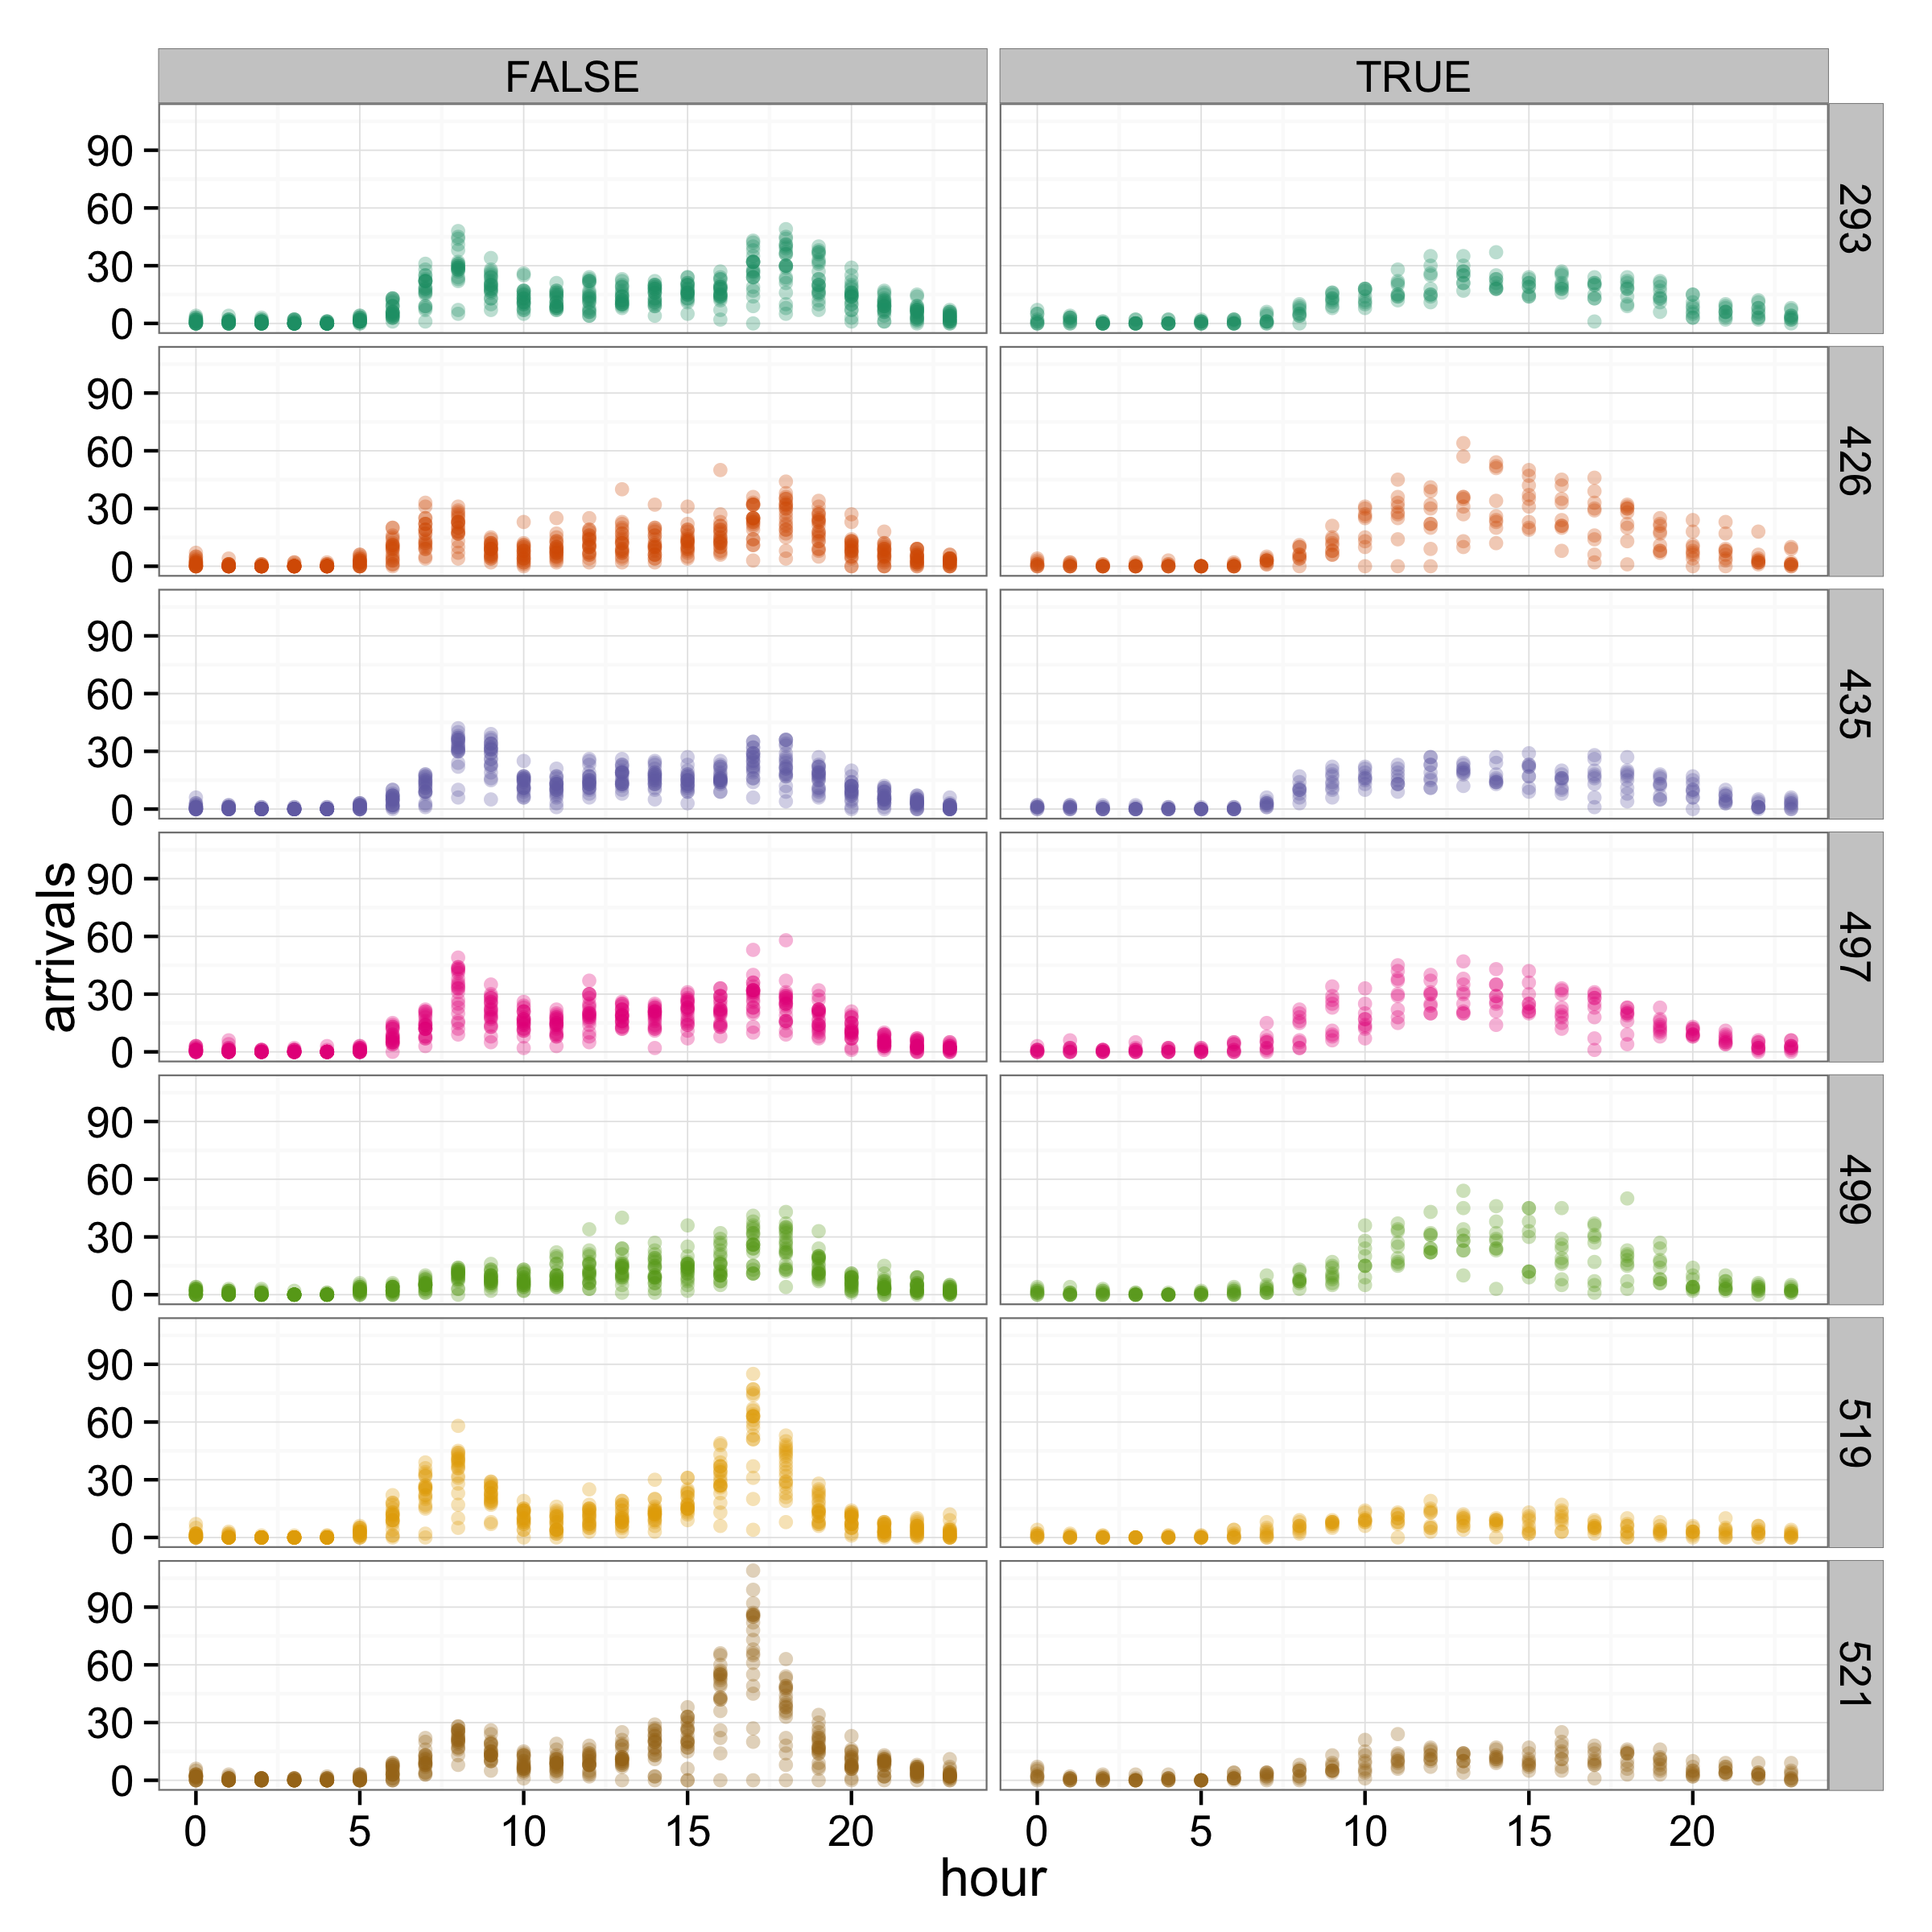
\includegraphics{../fig/top7_average_day.png}

\begin{center}\rule{0.5\linewidth}{\linethickness}\end{center}

\section{fitting GLMs and extracting prediction
error}\label{fitting-glms-and-extracting-prediction-error}

We are considering three increasingly complex models of the arrival
behavior. In order to compare three candidate models' prediction error,
we'll use K-fold cross validation, where we use the same folds for all
three models.

First, we the load the data and make our K-fold test sets (and
implicitly, our training sets):

\begin{Shaded}
\begin{Highlighting}[]
\KeywordTok{load}\NormalTok{(}\KeywordTok{url}\NormalTok{(}\StringTok{"http://www.stat.colostate.edu/~scharfh/CSP_parallel/data/arrivals_subset.RData"}\NormalTok{))}
\NormalTok{K <-}\StringTok{ }\DecValTok{50}
\NormalTok{N <-}\StringTok{ }\KeywordTok{dim}\NormalTok{(arrivals.sub)[}\DecValTok{1}\NormalTok{]}

\NormalTok{## for convenience kill off 8 observations (we have 5208) and make cv test sets}
\KeywordTok{set.seed}\NormalTok{(}\DecValTok{1985}\NormalTok{)}
\NormalTok{discarded <-}\StringTok{ }\KeywordTok{sample}\NormalTok{(}\DecValTok{1}\NormalTok{:N, }\DataTypeTok{size =} \DecValTok{8}\NormalTok{)}
\NormalTok{cv.test.sets <-}\StringTok{ }\KeywordTok{matrix}\NormalTok{(}\KeywordTok{sample}\NormalTok{((}\DecValTok{1}\NormalTok{:N)[-discarded], }\DataTypeTok{size =} \NormalTok{N -}\StringTok{ }\DecValTok{8}\NormalTok{), }\DataTypeTok{ncol =} \NormalTok{K)}
\end{Highlighting}
\end{Shaded}

Next, we build a function to fit the data to the training sets and
extract the corresponding estimate of prediciton error. This should
still be familiar code, no new packages yet.

\begin{Shaded}
\begin{Highlighting}[]
\NormalTok{lq.loss <-}\StringTok{ }\NormalTok{function(y, y.hat, }\DataTypeTok{q =} \DecValTok{1}\NormalTok{) \{(}\KeywordTok{abs}\NormalTok{(y -}\StringTok{ }\NormalTok{y.hat))^q\}}
\NormalTok{get.errs <-}\StringTok{ }\NormalTok{function(}\DataTypeTok{test.set =} \OtherTok{NULL}\NormalTok{,}
                     \DataTypeTok{discarded =} \OtherTok{NULL}\NormalTok{,}
                     \DataTypeTok{q =} \DecValTok{1}\NormalTok{) \{}
    \NormalTok{sml.glm <-}\StringTok{ }\KeywordTok{glm}\NormalTok{(arrivals ~}
\StringTok{                   }\KeywordTok{bs}\NormalTok{(hour, }\DataTypeTok{degree =} \DecValTok{4}\NormalTok{)}
                   \NormalTok{+}\StringTok{ }\NormalTok{weekend}
                   \NormalTok{+}\StringTok{ }\KeywordTok{as.factor}\NormalTok{(id),}
                   \DataTypeTok{data =} \NormalTok{arrivals.sub[-}\KeywordTok{c}\NormalTok{(discarded, test.set), ],}
                   \DataTypeTok{family =} \StringTok{"poisson"}\NormalTok{)}
    \NormalTok{med.glm <-}\StringTok{ }\KeywordTok{glm}\NormalTok{(arrivals ~}
\StringTok{                   }\KeywordTok{bs}\NormalTok{(hour, }\DataTypeTok{degree =} \DecValTok{4}\NormalTok{)*weekend}
                   \NormalTok{+}\StringTok{ }\KeywordTok{as.factor}\NormalTok{(id),}
                   \DataTypeTok{data =} \NormalTok{arrivals.sub[-}\KeywordTok{c}\NormalTok{(discarded, test.set), ],}
                   \DataTypeTok{family =} \StringTok{"poisson"}\NormalTok{)}
    \NormalTok{big.glm <-}\StringTok{ }\KeywordTok{glm}\NormalTok{(arrivals ~}
\StringTok{                   }\KeywordTok{bs}\NormalTok{(hour, }\DataTypeTok{degree =} \DecValTok{4}\NormalTok{)*weekend}
                   \NormalTok{+}\StringTok{ }\KeywordTok{bs}\NormalTok{(hour, }\DataTypeTok{degree =} \DecValTok{4}\NormalTok{)*}\KeywordTok{as.factor}\NormalTok{(id),}
                   \DataTypeTok{data =} \NormalTok{arrivals.sub[-}\KeywordTok{c}\NormalTok{(discarded, test.set), ],}
                   \DataTypeTok{family =} \StringTok{"poisson"}\NormalTok{)}
    \NormalTok{sml.err <-}\StringTok{ }\KeywordTok{mean}\NormalTok{(}\KeywordTok{lq.loss}\NormalTok{(}\KeywordTok{predict}\NormalTok{(}\DataTypeTok{object =} \NormalTok{sml.glm,}
                                    \DataTypeTok{newdata =} \NormalTok{arrivals.sub[test.set, -}\DecValTok{7}\NormalTok{],}
                                    \DataTypeTok{type =} \StringTok{"response"}\NormalTok{),}
                            \NormalTok{arrivals.sub[test.set, }\DecValTok{7}\NormalTok{],}
                            \DataTypeTok{q =} \NormalTok{q))}
    \NormalTok{med.err <-}\StringTok{ }\KeywordTok{mean}\NormalTok{(}\KeywordTok{lq.loss}\NormalTok{(}\KeywordTok{predict}\NormalTok{(}\DataTypeTok{object =} \NormalTok{med.glm,}
                                    \DataTypeTok{newdata =} \NormalTok{arrivals.sub[test.set, -}\DecValTok{7}\NormalTok{],}
                                    \DataTypeTok{type =} \StringTok{"response"}\NormalTok{),}
                            \NormalTok{arrivals.sub[test.set, }\DecValTok{7}\NormalTok{],}
                            \DataTypeTok{q =} \NormalTok{q))}
    \NormalTok{big.err <-}\StringTok{ }\KeywordTok{mean}\NormalTok{(}\KeywordTok{lq.loss}\NormalTok{(}\KeywordTok{predict}\NormalTok{(}\DataTypeTok{object =} \NormalTok{big.glm,}
                                    \DataTypeTok{newdata =} \NormalTok{arrivals.sub[test.set, -}\DecValTok{7}\NormalTok{],}
                                    \DataTypeTok{type =} \StringTok{"response"}\NormalTok{),}
                            \NormalTok{arrivals.sub[test.set, }\DecValTok{7}\NormalTok{],}
                            \DataTypeTok{q =} \NormalTok{q))}
    \KeywordTok{return}\NormalTok{(}\KeywordTok{c}\NormalTok{(sml.err, med.err, big.err))}
\NormalTok{\}}
\end{Highlighting}
\end{Shaded}

The fits using all the data look like:
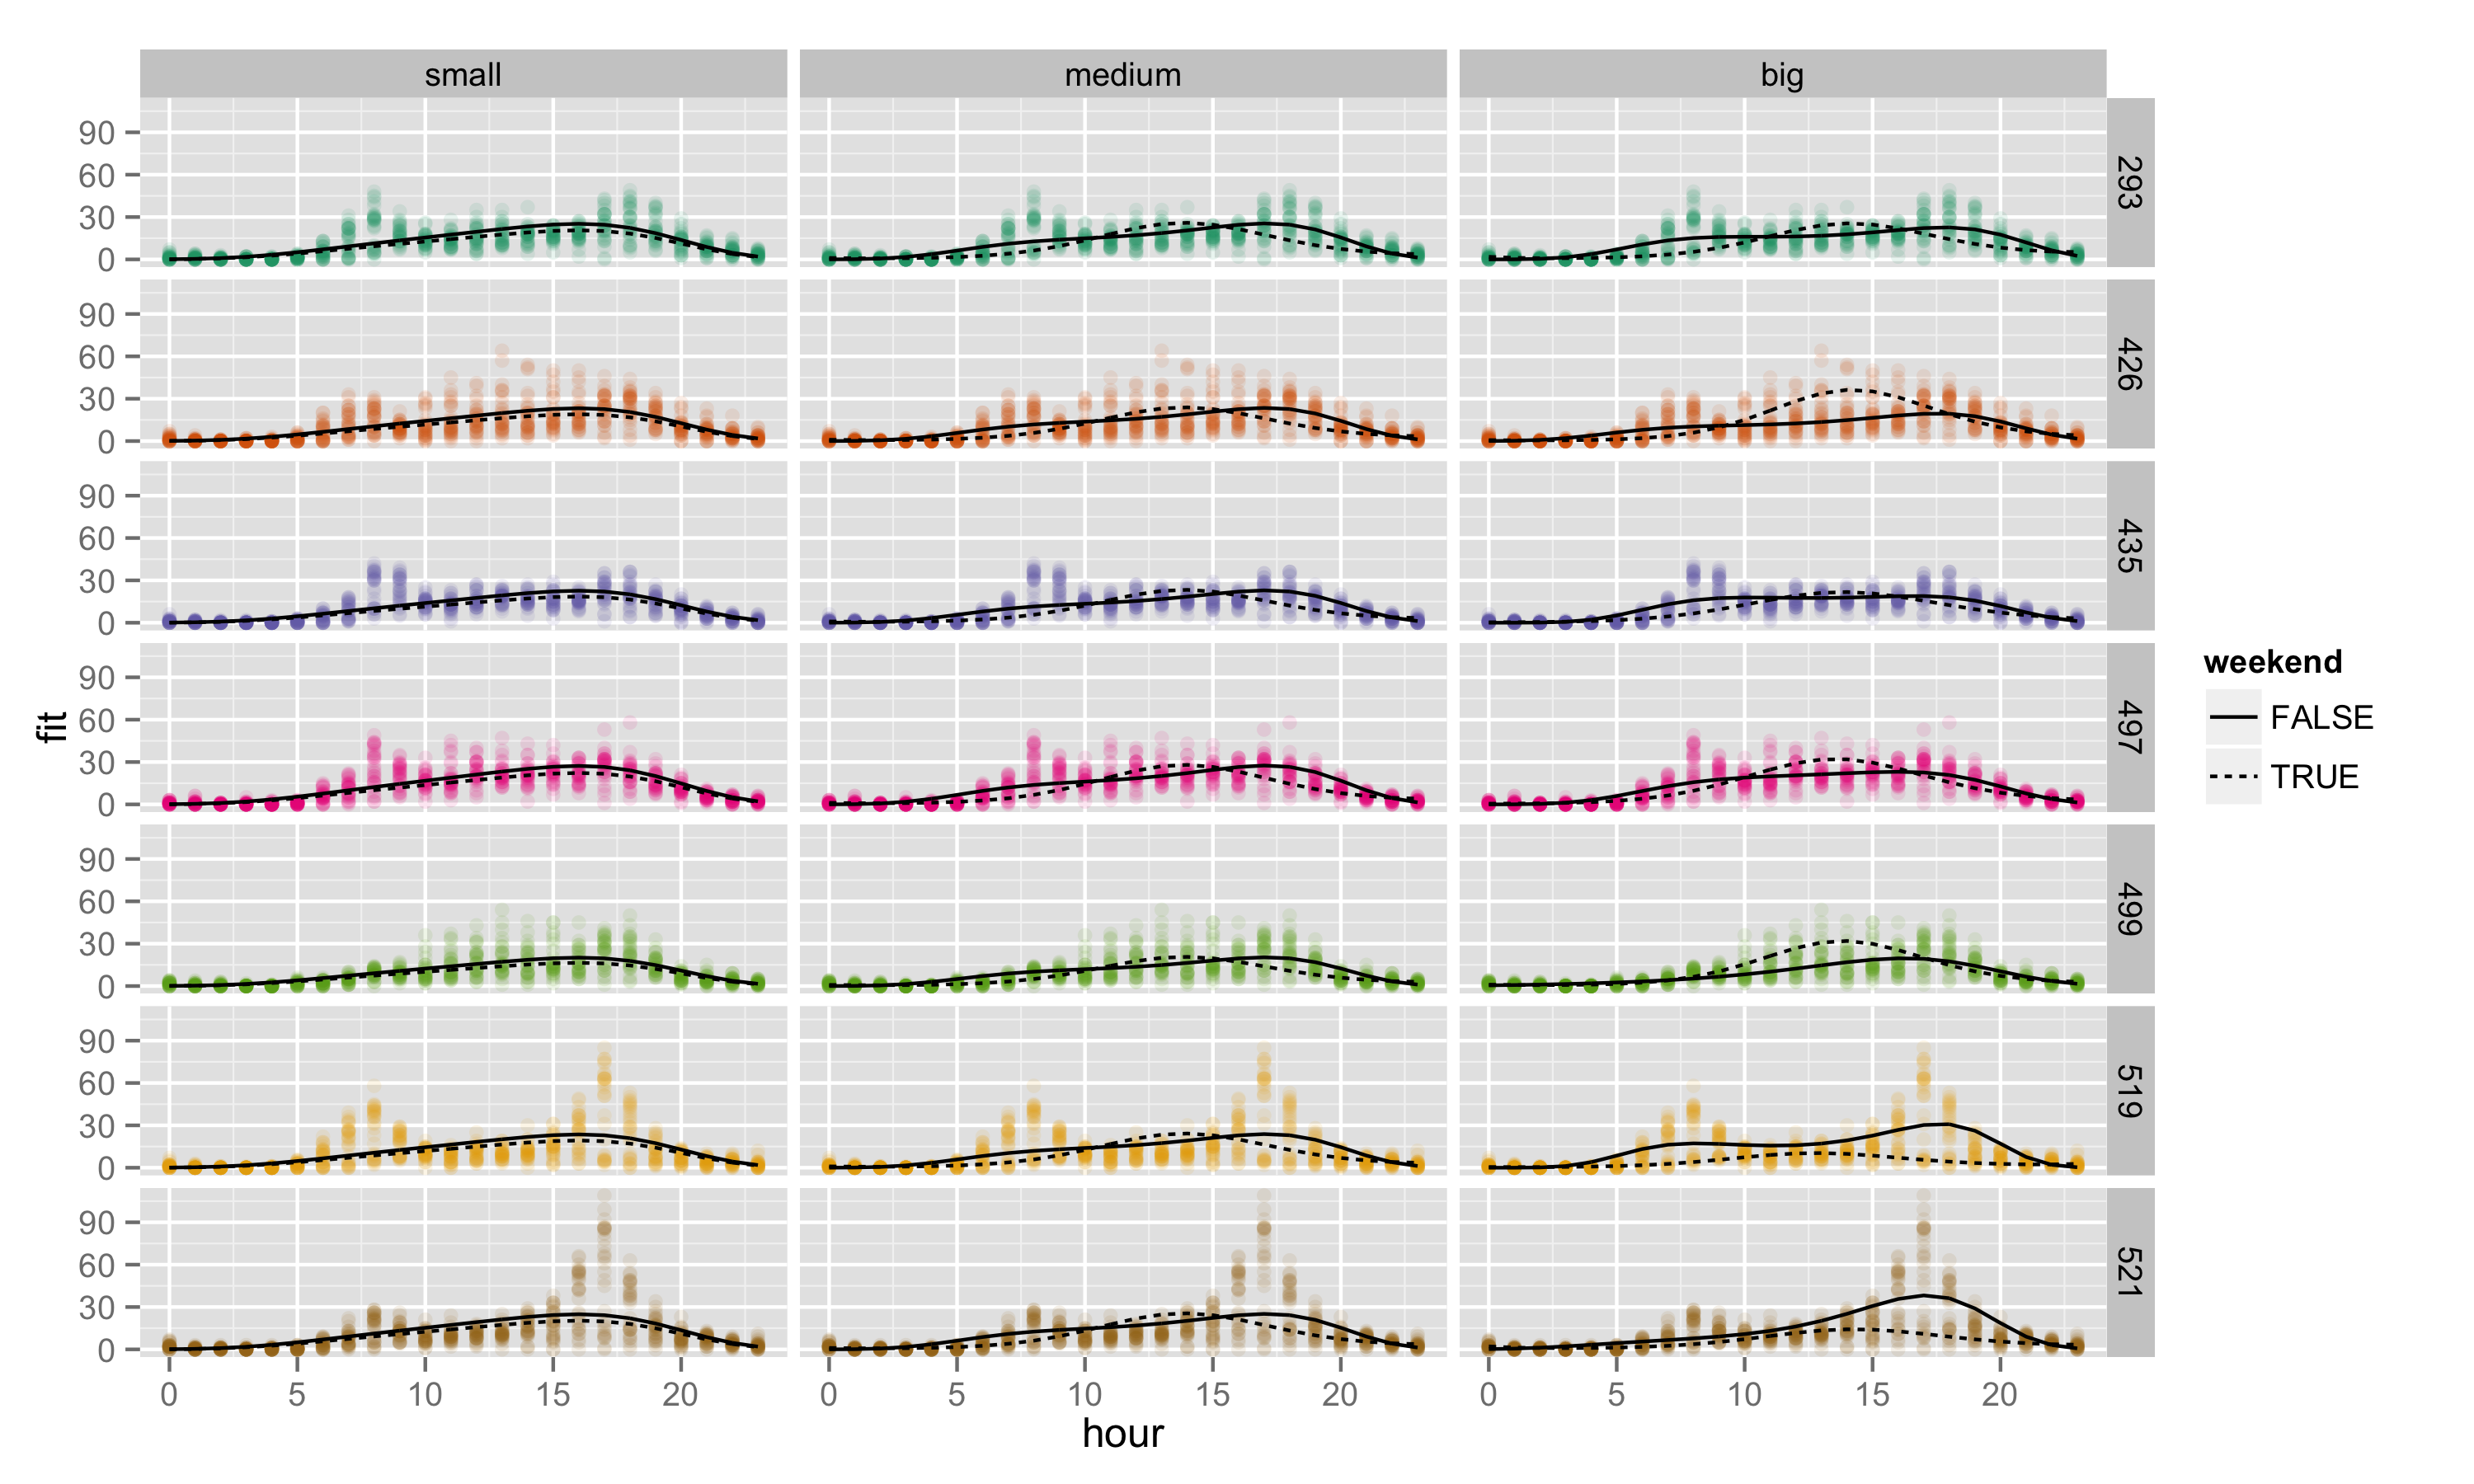
\includegraphics{../fig/fit_all.png}

\subsection{K-fold CV with a for loop}\label{k-fold-cv-with-a-for-loop}

Using a naive for loop, we could implement this as:

\begin{Shaded}
\begin{Highlighting}[]
\NormalTok{err.for <-}\StringTok{ }\OtherTok{NULL}
\KeywordTok{system.time}\NormalTok{(}
    \NormalTok{for (i in }\DecValTok{1}\NormalTok{:K) \{}
        \NormalTok{err.for <-}\StringTok{ }\KeywordTok{cbind}\NormalTok{(err.for, }\KeywordTok{get.errs}\NormalTok{(}\DataTypeTok{test.set =} \NormalTok{cv.test.sets[, i],}
                                           \DataTypeTok{discarded =} \NormalTok{discarded,}
                                           \DataTypeTok{q =} \DecValTok{1}\NormalTok{))}
        \NormalTok{\}}
    \NormalTok{)}
\end{Highlighting}
\end{Shaded}

\begin{verbatim}
##    user  system elapsed 
##  18.912   0.809  20.039
\end{verbatim}

\subsection{K-fold CV with an apply
function}\label{k-fold-cv-with-an-apply-function}

If you're good with \texttt{apply()} functions you might upgrade
(slightly) to

\begin{Shaded}
\begin{Highlighting}[]
\NormalTok{## apply version}
\KeywordTok{system.time}\NormalTok{(}
    \NormalTok{err.apply <-}\StringTok{ }\KeywordTok{sapply}\NormalTok{(}\DataTypeTok{X =} \DecValTok{1}\NormalTok{:K, }
                        \DataTypeTok{FUN =} \NormalTok{function(i) \{}
                            \KeywordTok{get.errs}\NormalTok{(}\DataTypeTok{test.set =} \NormalTok{cv.test.sets[, i],}
                                     \DataTypeTok{discarded =} \NormalTok{discarded,}
                                     \DataTypeTok{q =} \DecValTok{1}\NormalTok{)}
                            \NormalTok{\}}
                        \NormalTok{)}
    \NormalTok{)}
\end{Highlighting}
\end{Shaded}

\begin{verbatim}
##    user  system elapsed 
##  20.643   1.006  23.400
\end{verbatim}

Neither of the first two methods take advantage of multiple processors.
While the \texttt{apply()} functions avoid the inherently sluggish
nature of for loops in \texttt{R}, they are still ignorant of the
processor structure. We want to chop the job into halves, fourths, etc.
and use the \emph{whole} computer!

\subsection{K-fold CV with a foreach
loop}\label{k-fold-cv-with-a-foreach-loop}

Here is the same computation written with a \texttt{foreach} loop

\begin{Shaded}
\begin{Highlighting}[]
\NormalTok{## foreach version}
\KeywordTok{library}\NormalTok{(foreach)}
\KeywordTok{library}\NormalTok{(doParallel)}
\end{Highlighting}
\end{Shaded}

\begin{verbatim}
## Loading required package: iterators
## Loading required package: parallel
\end{verbatim}

\begin{Shaded}
\begin{Highlighting}[]
\KeywordTok{registerDoParallel}\NormalTok{(}\DataTypeTok{cl =} \DecValTok{2}\NormalTok{)}
\KeywordTok{system.time}\NormalTok{(}
    \NormalTok{err.foreach <-}\StringTok{ }\KeywordTok{foreach}\NormalTok{(}\DataTypeTok{i=}\DecValTok{1}\NormalTok{:K,}
                           \DataTypeTok{.inorder =} \OtherTok{FALSE}\NormalTok{,}
                           \DataTypeTok{.combine =} \StringTok{"cbind"}\NormalTok{) %dopar%}\StringTok{ }\NormalTok{\{}
                               \KeywordTok{get.errs}\NormalTok{(}\DataTypeTok{test.set =} \NormalTok{cv.test.sets[, i],}
                                        \DataTypeTok{discarded =} \NormalTok{discarded,}
                                        \DataTypeTok{q =} \DecValTok{1}\NormalTok{)}
                               \NormalTok{\}}
    \NormalTok{)}
\end{Highlighting}
\end{Shaded}

\begin{verbatim}
##    user  system elapsed 
##  10.612   0.534  11.488
\end{verbatim}

\section{components of a foreach
loop}\label{components-of-a-foreach-loop}

Note that despite the syntactically similar structure,
\texttt{foreach()} is a different animal than \texttt{for}. It is a
function with several important arguments. The first is the object we
iterate over and functions like the \texttt{(i in 1:K)} in the for loop.
The rest of the structure is new:

\begin{itemize}
\itemsep1pt\parskip0pt\parsep0pt
\item
  \texttt{\%\_\_\_\%}

  \begin{itemize}
  \itemsep1pt\parskip0pt\parsep0pt
  \item
    \texttt{\%do\%} performs the calculations in order and uses only one
    processor.
  \item
    \texttt{\%dopar\%} is what we generally wish to use.
  \item
    \texttt{\%dorng\%} will be discussed later, and is required for
    procedures that use randomly generated numbers.
  \item
    \texttt{\%:\%} can be used for nesting loops, which we'll see in an
    example at the end of the tutorial.
  \end{itemize}
\item
  arguments

  \begin{itemize}
  \itemsep1pt\parskip0pt\parsep0pt
  \item
    \texttt{.combine} can take on the intuitive values
    \texttt{\textquotesingle{}c\textquotesingle{}},
    \texttt{\textquotesingle{}cbind\textquotesingle{}}, or
    \texttt{\textquotesingle{}+\textquotesingle{}} as well as more
    complex functions and tells \texttt{foreach} how to combine the
    outputs from each iteration. The default is to return a list.
  \item
    \texttt{.inorder} is a \texttt{TRUE}/\texttt{FALSE} argument. In
    general, it is better to change this from the default of
    \texttt{TRUE} to \texttt{FALSE} whenever possible.
  \end{itemize}
\item
  Notice that unlike \texttt{apply()} functions, the \texttt{foreach}
  takes an expression (in braces after \texttt{\%dopar\%}) instead of a
  function.
\end{itemize}

\section{results}\label{results}

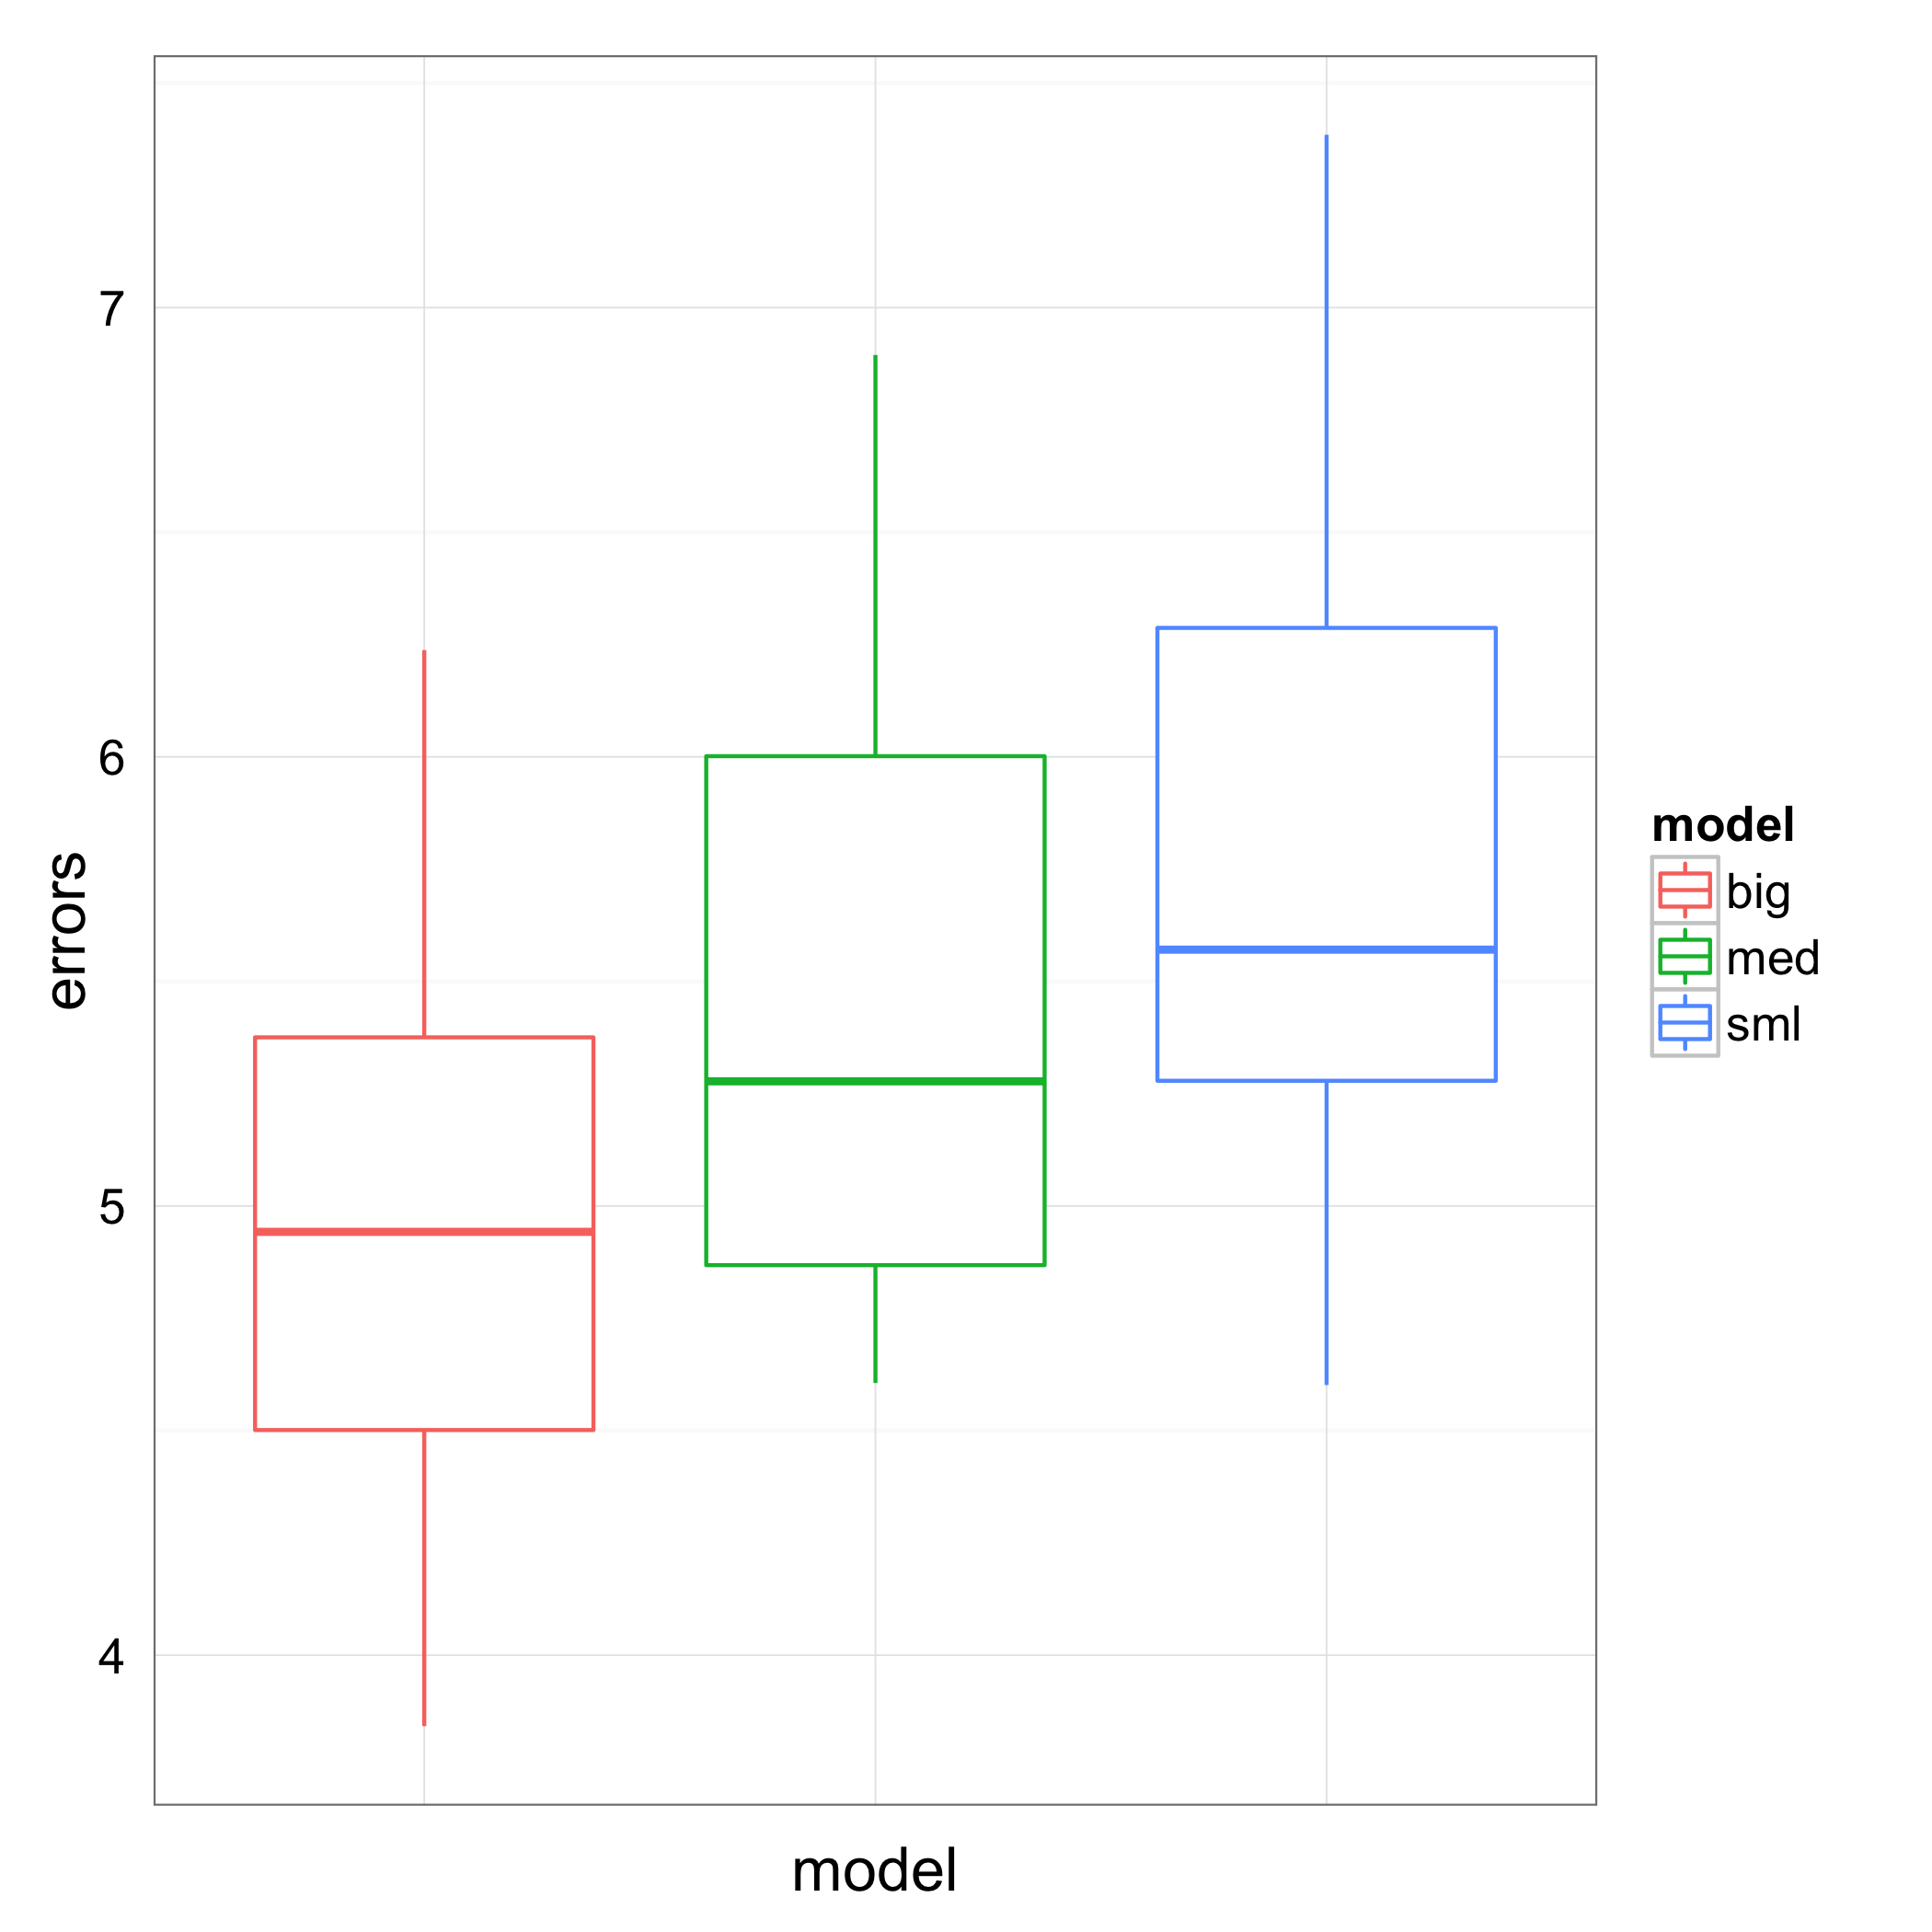
\includegraphics{../fig/error_boxplots.png}

\section{additional topics}\label{additional-topics}

\subsection{iterators}\label{iterators}

Sometimes the list or vector that we are iterating over (in the above
case, the vector \texttt{1:K}) can be a very large object. In our case
the vector is quite reasonable in size, but the object we are iterating
over could instead be a multi-dimensional object with many values and a
high level of precision. In this case, we'd be storing a complete copy
of this massive object for each processor, which could potentially fill
up our memory and slow things down. We could save memory by only keeping
the piece of our list we need for a given calculation as they are
computed, and dumping the rest. This is the idea behind the
\texttt{iterators} package in R.

Here is our same example with an iterator instead of a list.

\begin{Shaded}
\begin{Highlighting}[]
\KeywordTok{library}\NormalTok{(iterators)}
\KeywordTok{registerDoParallel}\NormalTok{(}\DataTypeTok{cl =} \DecValTok{2}\NormalTok{)}
\KeywordTok{system.time}\NormalTok{(}
    \NormalTok{err.foreach.iter <-}\StringTok{ }\KeywordTok{foreach}\NormalTok{(}\DataTypeTok{x =} \KeywordTok{iter}\NormalTok{(cv.test.sets, }\DataTypeTok{by =} \StringTok{"col"}\NormalTok{),}
                               \DataTypeTok{.inorder =} \OtherTok{FALSE}\NormalTok{,}
                               \DataTypeTok{.combine =} \StringTok{"cbind"}\NormalTok{) %dopar%}\StringTok{ }\NormalTok{\{}
                                   \KeywordTok{get.errs}\NormalTok{(}\DataTypeTok{test.set =} \NormalTok{x,}
                                            \DataTypeTok{discarded =} \NormalTok{discarded,}
                                            \DataTypeTok{q =} \DecValTok{1}\NormalTok{)}
                                   \NormalTok{\}}
    \NormalTok{)}
\end{Highlighting}
\end{Shaded}

\begin{verbatim}
##    user  system elapsed 
##   21.54    1.07   12.07
\end{verbatim}

Iterators can also be used to keep from ever having to store even a
single copy of the object. For more on these, see
\href{http://cran.r-project.org/web/packages/foreach/vignettes/foreach.pdf}{Using
the foreach package} and
\href{http://cran.r-project.org/web/packages/iterators/vignettes/iterators.pdf}{Using
the iterators package}.

\subsection{random numbers}\label{random-numbers}

When parallelizing a process which generates random numbers we need to
be careful, since we aren't guaranteed that \texttt{foreach} will handle
this properly. We could wind up getting numbers that aren't in fact
random! Moreover, if we want to be able to reproduce an analysis which
uses a random number generator, the usual \texttt{set.seed()} isn't
guaranteed to work.

Fortunately, there is \texttt{doRNG}. There are many ways to implement
this package, the two easiest of which are:

\begin{Shaded}
\begin{Highlighting}[]
\KeywordTok{library}\NormalTok{(doRNG)}
\end{Highlighting}
\end{Shaded}

\begin{verbatim}
## Loading required package: rngtools
## Loading required package: pkgmaker
## Loading required package: registry
\end{verbatim}

\begin{Shaded}
\begin{Highlighting}[]
\KeywordTok{registerDoParallel}\NormalTok{(}\DataTypeTok{cl =} \DecValTok{2}\NormalTok{)}
\NormalTok{blah1 <-}\StringTok{ }\KeywordTok{foreach}\NormalTok{(}\DataTypeTok{x =} \DecValTok{1}\NormalTok{:}\DecValTok{10}\NormalTok{, }
                 \DataTypeTok{.options.RNG =} \DecValTok{1985}\NormalTok{,}
                 \DataTypeTok{.combine =} \StringTok{'c'}\NormalTok{) %dorng%}\StringTok{ }\NormalTok{\{}
                     \KeywordTok{rnorm}\NormalTok{(}\DecValTok{1}\NormalTok{)}
                     \NormalTok{\}}
\end{Highlighting}
\end{Shaded}

and

\begin{Shaded}
\begin{Highlighting}[]
\KeywordTok{registerDoParallel}\NormalTok{(}\DataTypeTok{cl =} \DecValTok{2}\NormalTok{)}
\KeywordTok{registerDoRNG}\NormalTok{(}\DataTypeTok{seed =} \DecValTok{1985}\NormalTok{)}
\NormalTok{blah2 <-}\StringTok{ }\KeywordTok{foreach}\NormalTok{(}\DataTypeTok{x =} \DecValTok{1}\NormalTok{:}\DecValTok{10}\NormalTok{,}
                 \DataTypeTok{.combine =} \StringTok{'c'}\NormalTok{) %dopar%}\StringTok{ }\NormalTok{\{}
    \KeywordTok{rnorm}\NormalTok{(}\DecValTok{1}\NormalTok{)}
    \NormalTok{\}}
\end{Highlighting}
\end{Shaded}

Note that this gives reproducible results!

\begin{Shaded}
\begin{Highlighting}[]
\KeywordTok{sum}\NormalTok{(blah1 !=}\StringTok{ }\NormalTok{blah2) }
\end{Highlighting}
\end{Shaded}

\begin{verbatim}
## [1] 0
\end{verbatim}

\subsection{packages that support
foreach}\label{packages-that-support-foreach}

Some packages come with parallel functionality built in via
\texttt{foreach}.

\begin{itemize}
\itemsep1pt\parskip0pt\parsep0pt
\item
  \texttt{glmnet}
\item
  \texttt{gam}
\item
  \texttt{ggmcmc}
\item
  \texttt{plyr}
\item
  many others: see
  \href{http://cran.r-project.org/web/packages/foreach/index.html}{reverse
  suggests}
\end{itemize}

\section{{exercise}: fix up the following
code}\label{exercise-fix-up-the-following-code}

The following calculation wouldn't typically require parallelization
because it isn't a huge task, however we use it for practice's sake.

Suppose we wish to figure out which day in May had the most combined
arrivals across these seven stations. Here's a function to get started,
you're welcome to scrap it for your own, or use it and fill in the gaps
in what follows.

\begin{Shaded}
\begin{Highlighting}[]
\NormalTok{sum.arrivals <-}\StringTok{ }\NormalTok{function(}\DataTypeTok{date =} \OtherTok{NULL}\NormalTok{,}
                         \DataTypeTok{id =} \OtherTok{NULL}\NormalTok{)\{}
    \NormalTok{sum.arr <-}\StringTok{ }\KeywordTok{sum}\NormalTok{(arrivals.sub$arrivals[arrivals.sub$date ==}\StringTok{ }\NormalTok{date &}
\StringTok{                                         }\NormalTok{arrivals.sub$id ==}\StringTok{ }\NormalTok{id])}
    \KeywordTok{return}\NormalTok{(sum.arr)}
\NormalTok{\}}
\end{Highlighting}
\end{Shaded}

The following code needs some help. When nesting \texttt{foreach} loops
(\href{http://cran.r-project.org/web/packages/foreach/vignettes/nested.pdf}{see
this vignette}), we need to use \texttt{\%:\%}. Fill in the missing
parts to make the code work.

\begin{Shaded}
\begin{Highlighting}[]
\KeywordTok{system.time}\NormalTok{(}
    \KeywordTok{registerDoParallel}\NormalTok{(}\DataTypeTok{cl =} \DecValTok{2}\NormalTok{)}
    \NormalTok{busiest <-}\StringTok{ }\KeywordTok{foreach}\NormalTok{(}\DataTypeTok{date =} \NormalTok{___,}
                       \DataTypeTok{._______ =} \OtherTok{FALSE}\NormalTok{,}
                       \DataTypeTok{.combine =} \NormalTok{___) %:%}
\StringTok{                           }\KeywordTok{foreach}\NormalTok{(}\DataTypeTok{id =} \KeywordTok{unique}\NormalTok{(arrivals.sub$id),}
                                   \DataTypeTok{.inorder =} \NormalTok{______,}
                                   \DataTypeTok{.combine =} \NormalTok{___) %_____%}\StringTok{ }\NormalTok{\{}
                                       \KeywordTok{sum.arrivals}\NormalTok{(}\DataTypeTok{date =} \NormalTok{date,}
                                                    \DataTypeTok{id =} \NormalTok{id)}
                                   \NormalTok{\}}
                       \ErrorTok{\}}
    \NormalTok{)}
\KeywordTok{which}\NormalTok{(busiest==}\KeywordTok{max}\NormalTok{(busiest))    }
\end{Highlighting}
\end{Shaded}

For something this small, the overhead of managing the parallelization
means a regular nested for loop is quicker.

\begin{Shaded}
\begin{Highlighting}[]
\NormalTok{sum.arrivals <-}\StringTok{ }\NormalTok{function(}\DataTypeTok{date =} \OtherTok{NULL}\NormalTok{,}
                         \DataTypeTok{id =} \OtherTok{NULL}\NormalTok{)\{}
    \NormalTok{sum.arr <-}\StringTok{ }\KeywordTok{sum}\NormalTok{(arrivals.sub$arrivals[arrivals.sub$date ==}\StringTok{ }\NormalTok{date &}
\StringTok{                                         }\NormalTok{arrivals.sub$id ==}\StringTok{ }\NormalTok{id])}
    \KeywordTok{return}\NormalTok{(sum.arr)}
\NormalTok{\}}
\NormalTok{busiest.for <-}\StringTok{ }\KeywordTok{rep}\NormalTok{(}\DecValTok{0}\NormalTok{, }\DecValTok{31}\NormalTok{)}
\KeywordTok{system.time}\NormalTok{(}
    \NormalTok{for(date in }\DecValTok{1}\NormalTok{:}\DecValTok{31}\NormalTok{)\{}
        \NormalTok{for(id in }\KeywordTok{unique}\NormalTok{(arrivals.sub$id))\{}
            \NormalTok{busiest.for[date] <-}\StringTok{ }\KeywordTok{sum}\NormalTok{(busiest.for[date],}
                                     \KeywordTok{sum.arrivals}\NormalTok{(}\DataTypeTok{date =} \NormalTok{date, }\DataTypeTok{id =} \NormalTok{id))}
        \NormalTok{\}}
    \NormalTok{\}}
    \NormalTok{)}
\end{Highlighting}
\end{Shaded}

\begin{verbatim}
##    user  system elapsed 
##   0.073   0.004   0.078
\end{verbatim}

\begin{Shaded}
\begin{Highlighting}[]
\KeywordTok{which}\NormalTok{(busiest.for==}\KeywordTok{max}\NormalTok{(busiest.for))    }
\end{Highlighting}
\end{Shaded}

\begin{verbatim}
## [1] 20
\end{verbatim}

\section{{references}}\label{references}

\subsection{Other tutorials}\label{other-tutorials}

\href{http://cran.r-project.org/web/packages/doParallel/vignettes/gettingstartedParallel.pdf}{Getting
Started with doParallel and foreach}

\href{http://cran.r-project.org/web/packages/foreach/vignettes/foreach.pdf}{Using
the foreach package}

\href{http://cran.r-project.org/web/packages/iterators/vignettes/iterators.pdf}{Using
the iterators package}

\href{http://cran.r-project.org/web/packages/foreach/vignettes/nested.pdf}{Nesting
foreach loops}

\subsection{Data}\label{data-1}

\href{https://www.citibikenyc.com/system-data}{citibike system data}

\end{document}
